\chapter{量子谐振子}
\label{chap:harmonic-oscillator}

\section{量子谐振子的作用}
\label{sec:harmonic-role}

谐振子之所以重要,有多方面原因.在固体物理中,晶体可以建模为大量耦合谐振子的系统;利用“正规模”概念,该模型可化为具有不同频率的相互独立的一维谐振子.在量子力学中,不同正规模的激发称为声子.

自由量子场论同样可以看成一族耦合谐振子,只是场论中有无穷多个谐振子.即使是相互作用的量子场论,也常用谐振子的升降算子描述;在场论语境中,它们分别称为产生算子和湮灭算子.

分析谐振子还引出了量子力学的代数方法:用算子之间的代数关系(特别是对易关系)大幅取代微分方程,作为求解量子系统的手段.本章大部分工作在代数方法的小节中完成,剩余的解析问题在后两节处理.

\section{代数方法}
\label{sec:harmonic-algebraic}

本节只使用位置、动量算子的对易关系
\[
[X,P]=i\hbar I,
\label{eq:harmonic-xp-commutator}
\]
尽可能推导量子谐振子 Hamilton 算子的信息.这里 \([A,B]=AB-BA\) 是对易子.谐振子的 Hamilton 算子为
\[
\widehat H=\frac{P^{2}}{2m}+\frac{k}{2}X^{2},
\label{eq:harmonic-hamiltonian-k}
\]
其中 \(k>0\).我们希望只由 \(X,P\) 自伴且满足式~\eqref{eq:harmonic-xp-commutator} 这一事实,研究 \(\widehat H\) 的特征向量和特征值,而不使用它们的具体表达式.

严格说来,还隐含假设了某些定义域条件,即第~\ref{sec:harmonic-algebraic} 节中出现的向量属于相关算子的定义域.对通常作用在 \(L^{2}(\mathbb{R})\) 上的位置、动量算子,这些条件最终确实成立;一般满足对易关系的两个自伴算子则需要更细致的分析,第~14 章还会回到这一问题.

令 \(\omega=\sqrt{k/m}\),即相应经典谐振子的频率.将 \(k\) 换为 \(m\omega^{2}\),得到
\[
\widehat H=\frac{1}{2m}\left[P^{2}+(m\omega X)^{2}\right].
\label{eq:harmonic-hamiltonian-omega}
\]
定义降算子 \(a\) 和升算子 \(a^{*}\):
\[
a=\frac{m\omega X+iP}{\sqrt{2\hbar m\omega}},
\qquad
a^{*}=\frac{m\omega X-iP}{\sqrt{2\hbar m\omega}}.
\label{eq:harmonic-ladder-operators}
\]
它们之所以称为升降算子,是因为它们将分别升高和降低 Hamilton 算子的特征值.在量子场论中,类似的算子把 \(n\)-粒子空间映到 \((n+1)\)-粒子或 \((n-1)\)-粒子空间,因而称为产生和湮灭算子.

由于非交换算子满足
\[
(A-B)(A+B)=A^{2}-B^{2}+[A,B],
\]
使用式~\eqref{eq:harmonic-xp-commutator} 可得
\[
a^{*}a=\frac{1}{2\hbar m\omega}\left((m\omega X)^{2}+P^{2}+im\omega[X,P]\right)
=\frac{1}{\hbar\omega}\widehat H-\frac12I.
\]
所以
\[
\widehat H=\hbar\omega\left(a^{*}a+\frac12I\right).
\label{eq:harmonic-hamiltonian-ladder}
\]
右端的 \(\frac12I\) 是“量子修正”:对应的经典公式没有这一项.

只需研究 \(a^{*}a\) 的谱,再给特征值加上 \(1/2\) 并乘以 \(\hbar\omega\) 即可.直接计算
\[
[a,a^{*}]=I.
\label{eq:ladder-commutator}
\]
于是
\[
[a,a^{*}a]=a,
\qquad
[a^{*},a^{*}a]=-a^{*}.
\label{eq:ladder-number-commutators}
\]
算子 \(a^{*}a\) 自伴(至少对称),且非负,因为
\[
\langle\psi,a^{*}a\psi\rangle=\langle a\psi,a\psi\rangle\geq0.
\]

\begin{proposition}[升降算子改变特征值]\label{prop:ladder-shift}
若 \(\psi\) 是 \(a^{*}a\) 特征值 \(\lambda\) 的特征向量,则
\[
a^{*}a(a\psi)=(\lambda-1)a\psi,
\qquad
a^{*}a(a^{*}\psi)=(\lambda+1)a^{*}\psi.
\]
因此 \(a\psi\) 要么为零,要么是特征值 \(\lambda-1\) 的特征向量;\(a^{*}\psi\) 要么为零,要么是特征值 \(\lambda+1\) 的特征向量.
\end{proposition}

\begin{proof}
由式~\eqref{eq:ladder-number-commutators},
\[
a^{*}a(a\psi)=(a(a^{*}a)-a)\psi=(\lambda-1)a\psi.
\]
对 \(a^{*}\psi\) 使用第二个对易关系即可.
\end{proof}

若 \(a^{*}a\psi=\lambda\psi\),则
\[
\lambda\|\psi\|^{2}=\langle a\psi,a\psi\rangle\geq0,
\]
所以 \(\lambda\geq0\).假设 \(a^{*}a\) 至少有一个特征向量.反复施加降算子,不可能永远得到非零向量,因为那会产生负特征值.因此存在 \(N\geq0\),使 \(a^{N}\psi\neq0\) 而 \(a^{N+1}\psi=0\).令 \(\psi_{0}=a^{N}\psi\),则
\[
a\psi_{0}=0,
\qquad
a^{*}a\psi_{0}=0.
\]
这就是基态;再反复施加升算子即可得到正特征值.

\begin{theorem}[谐振子的代数谱结构]\label{thm:harmonic-algebraic-structure}
若 \(\psi_{0}\) 是满足 \(a\psi_{0}=0\) 的单位向量,令
\[
\psi_{n}:=(a^{*})^{n}\psi_{0},qquad n\geq0.
\]
则对所有 \(m,n\geq0\),
\[
a^{*}\psi_{n}=\psi_{n+1},
\qquad
a^{*}a\psi_{n}=n\psi_{n},
\qquad
\langle\psi_{n},\psi_{m}\rangle=n!\,\delta_{n,m},
\qquad
a\psi_{n+1}=(n+1)\psi_{n}.
\label{eq:harmonic-chain-relations}
\]
\end{theorem}

\begin{proof}
第一式是定义,第二式由命题~\ref{prop:ladder-shift} 和 \(a^{*}a\psi_{0}=0\) 得到.若 \(n\neq m\),自伴(甚至对称)算子的不同特征值特征向量正交.若 \(n=m\),归纳使用
\[
\|\psi_{n+1}\|^{2}=\langle a^{*}\psi_{n},a^{*}\psi_{n}\rangle
=\langle\psi_{n},aa^{*}\psi_{n}\rangle
=\langle\psi_{n},(a^{*}a+I)\psi_{n}\rangle
=(n+1)\|\psi_{n}\|^{2}.
\]
最后,\(a\psi_{n+1}=aa^{*}\psi_{n}=(a^{*}a+I)\psi_{n}=(n+1)\psi_{n}\).
\end{proof}

这些向量形成一个正交链,其范数为 \(\sqrt{n!}\),升算子把链向上移动,降算子把链向下移动.若它们的闭线性包不是整个 Hilbert 空间,则其正交补也在 \(a,a^{*}\) 及 \(a^{*}a\) 下不变,可以在正交补中重新找到另一个与 \(\psi_{0}\) 正交的基态.因此,若方程 \(a\psi=0\) 的解(相差常数倍)只有一个,就期待这些 \(\psi_{n}\) 构成整个空间的正交基.

\section{解析方法}
\label{sec:harmonic-analytic}

现在使用位置、动量算子的具体形式.令自然长度尺度
\[
D:=\sqrt{\frac{\hbar}{m\omega}},
\qquad
\widetilde x:=\frac{x}{D}.
\]
于是
\[
\frac{\mathrm{d}}{\mathrm{d}\widetilde x}=D\frac{\mathrm{d}}{\mathrm{d}x}.
\]
升降算子化为
\[
a=\frac{1}{\sqrt2}\left(\widetilde x+\frac{\mathrm{d}}{\mathrm{d}\widetilde x}\right),
\qquad
a^{*}=\frac{1}{\sqrt2}\left(\widetilde x-\frac{\mathrm{d}}{\mathrm{d}\widetilde x}\right).
\label{eq:harmonic-dimensionless-ladder}
\]
注意 \(m,\omega,\hbar\) 已从公式中消失.

方程 \(a\psi_{0}=0\) 的解为
\[
\psi_{0}(\widetilde x)=Ce^{-\widetilde x^{2}/2}.
\]
由归一化条件,取正的 \(C\) 得
\[
\psi_{0}(x)=\left(\frac{m\omega}{\pi\hbar}\right)^{1/4}
\exp\left(-\frac{m\omega}{2\hbar}x^{2}\right).
\label{eq:harmonic-ground-state}
\]

\begin{theorem}[谐振子的 Hermite 态]\label{thm:harmonic-hermite-states}
基态由式~\eqref{eq:harmonic-ground-state} 给出,激发态为
\[
\psi_{n}=H_{n}\psi_{0},
\label{eq:harmonic-excited-states}
\]
其中 \(H_{n}\) 是次数为 \(n\) 的多项式,递推定义为
\[
H_{0}(\widetilde x)=1,
\qquad
H_{n+1}(\widetilde x)=\frac{1}{\sqrt2}\left(2\widetilde xH_{n}(\widetilde x)-\frac{\mathrm{d}H_{n}}{\mathrm{d}\widetilde x}\right).
\]
它们除归一化约定外就是 Hermite 多项式.
\end{theorem}

\begin{proof}
当 \(n=0\) 时显然.若 \(\psi_{n}=H_{n}\psi_{0}\),则由式~\eqref{eq:harmonic-dimensionless-ladder},
\[
\begin{aligned}
\psi_{n+1}=a^{*}\psi_{n}
&=\frac{1}{\sqrt2}\left(\widetilde x-\frac{\mathrm{d}}{\mathrm{d}\widetilde x}\right)
\left(H_{n}(\widetilde x)Ce^{-\widetilde x^{2}/2}\right)\\
&=\frac{1}{\sqrt2}\left(2\widetilde xH_{n}(\widetilde x)-H_{n}'(\widetilde x)\right)\psi_{0}(\widetilde x)
=H_{n+1}\psi_{0}.
\end{aligned}
\]
\end{proof}

\begin{figure}[htbp]
\centering
\includegraphics[page=250,pagebox=cropbox,trim=126.23bp 268.32bp 135.85bp 66.58bp,clip,width=0.70\textwidth]{../input/source/Quantum Theory for Mathematicians(Brian C. Hall).pdf}
\caption{量子谐振子的基态、\(n=5\) 和 \(n=30\) 激发态;阴影表示经典允许区域.}
\label{fig:harmonic-states}
\end{figure}

图~\ref{fig:harmonic-states} 展示基态以及 \(n=5,30\) 的激发态,横轴是无量纲位置 \(\widetilde x\),阴影是经典允许区域.波函数在允许区域外快速衰减.高激发态中,允许区域中央的振荡频率最大,而两端的振幅最大;这反映了经典粒子在势能最小处动量最大,在转向点附近速度最慢、停留时间最长.

\section{定义域条件与完备性}
\label{sec:harmonic-domain-completeness}

代数分析并非完全严格,因为 \(a,a^{*},a^{*}a\) 都是无界算子,必须不断检查向量是否属于相关算子的定义域.对通常的位置、动量算子,式~\eqref{eq:harmonic-excited-states} 中的函数是“多项式乘 Gaussian”,属于 Schwartz 空间,因此属于任何有限个升降算子乘积的定义域;所以第~\ref{sec:harmonic-algebraic} 节中的关系在本例中确实成立.

\begin{theorem}[谐振子本征函数的完备性]\label{thm:harmonic-completeness}
函数
\[
\psi_{n}(x)=H_{n}(\widetilde x)\psi_{0}(x)
\]
构成 Hilbert 空间 \(L^{2}(\mathbb{R})\) 的正交基.
\end{theorem}

\begin{lemma}[指数乘 Gaussian 的多项式逼近]\label{lem:gaussian-exponential-series}
对任意 \(\alpha\in\mathbb{C}\),级数的部分和
\[
\sum_{n=0}^{\infty}\frac{\alpha^{n}\widetilde x^{n}}{n!}e^{-\widetilde x^{2}/2}
\]
在 \(L^{2}(\mathbb{R})\) 中收敛到
\[
e^{\alpha\widetilde x}e^{-\widetilde x^{2}/2}.
\]
\end{lemma}

\begin{proof}
余项的绝对值平方被
\[
\left(\sum_{n=0}^{\infty}\frac{|\alpha\widetilde x|^{n}}{n!}\right)^{2}e^{-\widetilde x^{2}}
=e^{2|\alpha||\widetilde x|}e^{-\widetilde x^{2}}
\]
控制,该函数可积.支配收敛定理给出结论.
\end{proof}

\begin{proof}[定理~\ref{thm:harmonic-completeness} 的证明]
升降算子把 Schwartz 空间映到自身,且对 Schwartz 函数分部积分给出
\[
\langle\phi,a\psi\rangle=\langle a^{*}\phi,\psi\rangle.
\]
基态和所有激发态都属于 Schwartz 空间,因此它们是正交的,并且是 Hamilton 算子的特征向量.

令 \(V\) 为这些函数的有限线性组合空间.由于 \(H_{n}\) 的次数为 \(n\),\(V\) 正好由形如
\[
p(\widetilde x)e^{-\widetilde x^{2}/2}
\]
的函数组成,其中 \(p\) 是多项式.由引理~\ref{lem:gaussian-exponential-series},对任意 \(k\in\mathbb{R}\),函数 \(e^{ik\widetilde x}e^{-\widetilde x^{2}/2}\) 属于 \(V\) 的 \(L^{2}\) 闭包.若 \(\psi\) 与 \(V\) 的闭包正交,则
\[
\int_{\mathbb{R}}e^{-ik\widetilde x}e^{-\widetilde x^{2}/2}\psi(\widetilde x)\,\mathrm{d}\widetilde x=0
\]
对所有 \(k\) 成立.Gaussian 属于 \(L^{\infty}\cap L^{2}\),与 \(\psi\in L^{2}\) 的乘积属于 \(L^{1}\cap L^{2}\),所以其 Fourier 变换恒为零.由 Plancherel 定理,Gaussian 与 \(\psi\) 的乘积为零,因而 \(\psi=0\) 几乎处处.故 \(V\) 稠密.
\end{proof}

\section{练习}
\label{sec:chapter11-exercises}

\begin{exercise}[升降算子的伴随]\label{ex:ladder-adjoint-schwartz}
证明对任意 Schwartz 函数 \(\phi,\psi\),有 \(\langle\phi,a\psi\rangle=\langle a^{*}\phi,\psi\rangle\).
\emph{提示:}在 \([-A,A]\) 上分部积分,证明边界项在 \(A\to\infty\) 时趋于零.
\end{exercise}

\begin{exercise}[Hermite 多项式递推关系]\label{ex:hermite-recurrences}
证明
\[
H_{n-1}(y)=\frac{1}{\sqrt{2n}}H_{n}'(y),
\qquad
H_{n+1}(y)=\frac{1}{\sqrt2}\left(2yH_{n}(y)-\sqrt{2n}H_{n-1}(y)\right).
\]
\emph{提示:}从 \(a\psi_{n}=n\psi_{n-1}\) 出发.
\end{exercise}

\begin{exercise}[Rodrigues 公式]\label{ex:hermite-rodrigues}
证明
\[
H_{n}(y)=(-1)^{n}2^{-n/2}e^{y^{2}}\frac{\mathrm{d}^{n}}{\mathrm{d}y^{n}}e^{-y^{2}}.
\]
\end{exercise}

\begin{exercise}[Hermite 多项式的零点]\label{ex:hermite-zeros}
证明 \(H_{n}\) 有 \(n\) 个互异实零点,且 \(H_{n}\) 与 \(H_{n-1}\) 的零点交错.
\begin{enumerate}[label=(\alph*)]
\item 验证 \(H_{1},H_{0}\) 的情形;
\item 假设归纳结论对 \(H_{n},H_{n-1}\) 成立,证明 \(H_{n+1}\) 在 \(H_{n}\) 的相邻零点之间至少有一个零点;
\item 证明 \(H_{n+1}\) 在 \(H_{n}\) 的最小零点以下和最大零点以上各有一个零点;
\item 推出 \(H_{n+1}\) 有 \(n+1\) 个与 \(H_{n}\) 交错的实零点.
\end{enumerate}
\end{exercise}

\begin{exercise}[激发态的期望值]\label{ex:harmonic-expectations}
令 \(\widetilde\psi_{n}=\psi_{n}/\|\psi_{n}\|\),\(\widetilde X=X/D\),\(D=\sqrt{\hbar/(m\omega)}\).证明
\[
\langle\widetilde X^{2}\rangle_{\widetilde\psi_{n}}=n+\frac12,
\qquad
\langle X\rangle_{\widetilde\psi_{n}}=0,
\]
且
\[
\Delta_{\widetilde\psi_{n}}X=\sqrt{\frac{\hbar}{m\omega}\left(n+\frac12\right)}.
\]
若 \(T,V\) 分别表示式~\eqref{eq:harmonic-hamiltonian-omega} 中的动能和势能项,证明
\[
\langle T\rangle_{\widetilde\psi_{n}}=\langle V\rangle_{\widetilde\psi_{n}}
=\frac12\hbar\omega\left(n+\frac12\right).
\]
\end{exercise}
